\documentclass[a4paper,10pt,DIV=14]{article}
\usepackage{graphicx}
\usepackage[utf8]{inputenc} % korrekte Darstellung von Umlauten u. Sonderzeichen
\usepackage[ngerman]{babel} % Sprachpaket, ngerman = neue deutsche Rechtschreibung
\usepackage{amsmath} % Setzen mathematischer Formeln
\usepackage{amsfonts} %mathbb
\usepackage{titlesec}
\usepackage{float}
\usepackage{caption}
\usepackage{fancyvrb}
\usepackage{siunitx}
\usepackage{booktabs}
\usepackage{enumitem}
\usepackage{tikz}
\usetikzlibrary{positioning}

\usepackage{tabularx}
\newcolumntype{L}[1]{>{\raggedright\arraybackslash}p{#1}} % linksbündig mit Breitenangabe
\newcolumntype{C}[1]{>{\centering\arraybackslash}p{#1}} % zentriert mit Breitenangabe
\newcolumntype{R}[1]{>{\raggedleft\arraybackslash}p{#1}} % rechtsbündig mit Breitenangabe

\newcommand{\gqq}[1]{\glqq{}#1\grqq{}}
\newcommand{\gq}[1]{\glq{}#1\grq{}}
\newcommand{\dg}[1]{#1^\circ}

\renewcommand{\thesection}{Aufgabe \arabic{section}:}
\renewcommand{\thesubsection}{\alph{subsection})}
\renewcommand{\thesubsubsection}{\roman{subsubsection}}

\titleformat{\subsection}
{\normalsize}{\thesubsection}{1em}{}


\captionsetup[figure]{labelformat=empty}

\begin{document}

\title{Graphische Datenverarbeitung WS17/18 \\ Theorieübung 3}
\author{
  Salmah Ahmad (2880011)
  \and
  Markus Höhn (1683303)
  \and
  Tobias Mertz (2274355)
  \and
  Steven Lamarr Reynolds (1620638)
  \and
  Sascha Zenglein (2487032)
}

\maketitle

\section{Räumliche Datenstrukturen (2 Punkte)}

\subsection{(1 Punkt)}
BSP-Baum:\\
\begin{tikzpicture}[sibling distance=5cm, level distance=1.8cm,
level 1/.style={sibling distance=3cm},
level 2/.style={sibling distance=1.5cm},  
  every node/.style = {shape=circle, rounded corners,
    draw, align=center,
%    top color=white, bottom color=blue!20
	}]]
  \node[minimum size=1cm] {A}
    child[minimum size=1cm] { node {$B_1$} 
    	child[minimum size=1cm] { node {$C_1$}
    		child[minimum size=1cm] { node {E}}
    		child[missing, minimum size=1cm] {node {}}
    	}
    	child[minimum size=1cm] { node {F}}
    }
    child[minimum size=1cm] { node {G}
      child[minimum size=1cm] { node {H}}
      child[minimum size=1cm] { node {D}
			child[minimum size=1cm] { node {$C_2$}}     
			child[minimum size=1cm] { node {$B_2$}}
		}
      };
\end{tikzpicture}

\subsection{(1 Punkt)}
Zeichenreihenfolge (Zuerst $\rightarrow$ Zuletzt):\\
H, G, $B_2$, D, $C_2$, A, $C_1$, E, $B_1$, F

\section{Projektionen (5 Punkte)}

\subsection{a)}
\subsubsection{i}
$f_l= \begin{pmatrix}
tan(\frac{\theta}{2})\cdot f \\
f \\
\end{pmatrix}$ \\
$f_r= \begin{pmatrix}
-tan(\frac{\theta}{2})\cdot f \\
f \\
\end{pmatrix}$ \\
$n_l= \begin{pmatrix}
tan(\frac{\theta}{2})\cdot n \\
n \\
\end{pmatrix}$ \\
$n_r= \begin{pmatrix}
-tan(\frac{\theta}{2})\cdot n \\
n \\
\end{pmatrix}$ 

\subsubsection{ii}

\begin{figure}[!htbp]
	\centering
	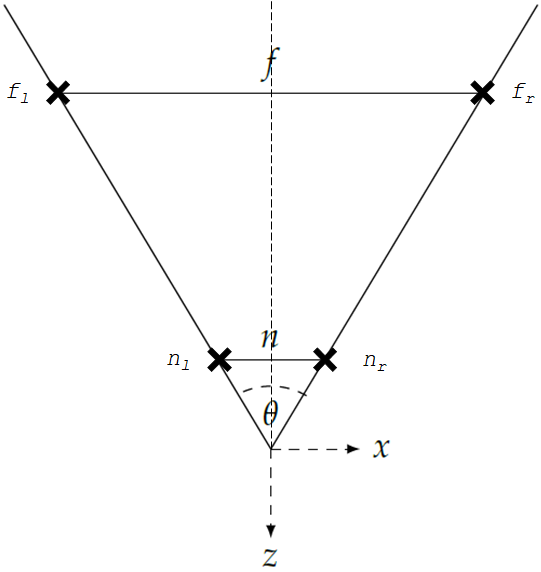
\includegraphics[width=1\linewidth]{frustum}
\end{figure}

$f_l= 
\begin{pmatrix}
	1 & 0 & 0  \\
	0 & 1+\frac{-f}{-n} & -f  \\
	0 & -\frac{1}{-n} & 0  \\
\end{pmatrix} \cdot
\begin{pmatrix}
	tan(\frac{\theta}{2})\cdot f \\
	f \\
	1 \\
\end{pmatrix}
= 
\begin{pmatrix}
	-\frac{-n}{f} \cdot tan(\frac{\theta}{2})\cdot f\\
	-\frac{-n}{f} \cdot(-f)-(-f-n) \\
	1 \\
\end{pmatrix}\\
= 
\begin{pmatrix}
	n \cdot tan(\frac{\theta}{2})\\
	f \\
	1 \\
\end{pmatrix}
$ \\
$f_r= 
\begin{pmatrix}
	1 & 0 & 0  \\
	0 & 1+\frac{-f}{-n} & -f  \\
	0 & -\frac{1}{-n} & 0  \\
\end{pmatrix} \cdot
\begin{pmatrix}
	-tan(\frac{\theta}{2})\cdot f \\
	f \\
	1 \\
\end{pmatrix}
=
\begin{pmatrix}
	-\frac{-n}{f} \cdot(-tan(\frac{\theta}{2}))\cdot f\\
	-\frac{-n}{f} \cdot(-f)-(-f-n) \\
	1 \\
\end{pmatrix}\\
= 
\begin{pmatrix}
	-n \cdot tan(\frac{\theta}{2})\\
	f \\
	1 \\
\end{pmatrix}
$ \\
$n_l= 
\begin{pmatrix}
	1 & 0 & 0  \\
	0 & 1+\frac{-f}{-n} & -f  \\
	0 & -\frac{1}{-n} & 0  \\
\end{pmatrix} \cdot
\begin{pmatrix}
	tan(\frac{\theta}{2})\cdot n \\
	n \\
	1 \\
\end{pmatrix}
=
\begin{pmatrix}
	-\frac{-n}{n} \cdot tan(\frac{\theta}{2})\cdot n\\
	-\frac{-n}{n} \cdot(-f)-(-f-n) \\
	1 \\
\end{pmatrix}\\
= 
\begin{pmatrix}
	n\cdot tan(\frac{\theta}{2})\\
	n \\
	1 \\
\end{pmatrix}
$ \\
$n_r= 
\begin{pmatrix}
	1 & 0 & 0  \\
	0 & 1+\frac{-f}{-n} & -f  \\
	0 & -\frac{1}{-n} & 0  \\
\end{pmatrix} \cdot
\begin{pmatrix}
	-tan(\frac{\theta}{2})\cdot n \\
	n \\
	1 \\
\end{pmatrix}
=
\begin{pmatrix}
	-\frac{-n}{n} \cdot(-tan(\frac{\theta}{2}))\cdot n\\
	-\frac{-n}{n} \cdot(-f)-(-f-n) \\
	1 \\
\end{pmatrix}\\
= 
\begin{pmatrix}
	-n \cdot tan(\frac{\theta}{2})\\
	n \\
	1 \\
\end{pmatrix}
$ \\

\subsubsection{iii}
$r = n \cdot tan(\frac{\theta}{2}) \qquad  l = -n \cdot tan(\frac{\theta}{2})
$\\
$f'_l=
P_0 \cdot f_l =
\begin{pmatrix}
    \frac{2}{r-l} & 0 & \frac{r+l}{l-r}\\
    0 & \frac{2}{f-n} & \frac{-f-n}{f-n}\\
    0 & 0 & 1\\
\end{pmatrix} \cdot
\begin{pmatrix}
    n \cdot tan(\frac{\theta}{2})\\
    f\\
    1\\
\end{pmatrix}$\\$ = 
\begin{pmatrix}
    \frac{1}{n \cdot tan(\frac{\theta}{2})} & 0 & 0\\
    0 & \frac{2}{f-n} & \frac{-f-n}{f-n}\\
    0 & 0 & 1\\
\end{pmatrix} \cdot
\begin{pmatrix}
    n \cdot tan(\frac{\theta}{2})\\
    f\\
    1
\end{pmatrix} =
\begin{pmatrix}
    1\\
    1\\
    1\\
\end{pmatrix}
$\\
$f'_r=
P_0 \cdot f_r =
\begin{pmatrix}
    \frac{1}{n \cdot tan(\frac{\theta}{2})} & 0 & 0\\
    0 & \frac{2}{f-n} & \frac{-f-n}{f-n}\\
    0 & 0 & 1\\
\end{pmatrix} \cdot
\begin{pmatrix}
    -n \cdot tan(\frac{\theta}{2})\\
    f\\
    1
\end{pmatrix} =
\begin{pmatrix}
    -1\\
    1\\
    1\\
\end{pmatrix}
$\\
$n'_l=
P_0 \cdot n_l =
\begin{pmatrix}
    \frac{1}{n \cdot tan(\frac{\theta}{2})} & 0 & 0\\
    0 & \frac{2}{f-n} & \frac{-f-n}{f-n}\\
    0 & 0 & 1\\
\end{pmatrix} \cdot
\begin{pmatrix}
    n \cdot tan(\frac{\theta}{2})\\
    n\\
    1
\end{pmatrix} =
\begin{pmatrix}
    1\\
    -1\\
    1\\
\end{pmatrix}
$\\
$n'_r=
P_0 \cdot n_r =
\begin{pmatrix}
    \frac{1}{n \cdot tan(\frac{\theta}{2})} & 0 & 0\\
    0 & \frac{2}{f-n} & \frac{-f-n}{f-n}\\
    0 & 0 & 1\\
\end{pmatrix} \cdot
\begin{pmatrix}
    -n \cdot tan(\frac{\theta}{2})\\
    n\\
    1
\end{pmatrix} =
\begin{pmatrix}
    -1\\
    -1\\
    1\\
\end{pmatrix}$\\

\subsection{b)}
\subsection{c)}
$z'_0 = 6$\\
$z'_1 = 6$\\
$z'_2 = 7$\\
$z'_3 = 5$\\
$z'_4 = 3$\\
$z'_5 = 3$
\begin{figure}[!htbp]
	\centering
	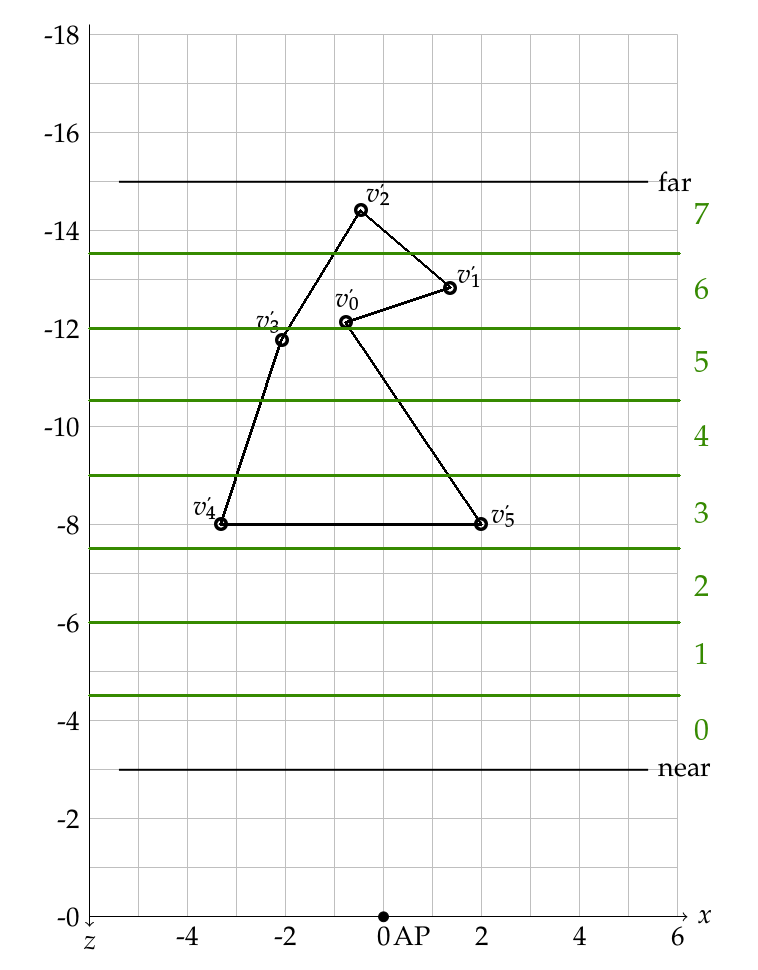
\includegraphics[width=1\linewidth]{2c}
\end{figure}
\subsection{d)}
\begin{align*}
    z' = f(z) &= z \cdot \left( 1 + \frac{f}{n} \right) -f\\
    z' + f &= z \cdot \left( 1 + \frac{f}{n} \right)\\
    \frac{z' + f}{1 + \frac{f}{n}} &= z = g(z')
\end{align*}
Tiefenwert 1:\\
$\left[ g(-4.5), g(-6) \right] = \left[ \frac{-4.5 - 15}{1 + \frac{15}{3}} , \frac{-6 - 15}{1 + \frac{15}{3}} \right] = \left[ -\frac{19.5}{6} , -\frac{21}{6} \right] = \left[ -3.25 , -3.5 \right]$\\
Tiefenwert 6:\\
$\left[ g(-12), g(-13.5) \right] = \left[ \frac{-12 - 15}{1 + \frac{15}{3}} , \frac{-13.5 - 15}{1 + \frac{15}{3}} \right] = \left[ -\frac{27}{6} , -\frac{28.5}{6} \right] = \left[ -4.5 , -4.75 \right]$

\newcommand*\BitAnd{\mathrel{\&}}
\newcommand*\BitOr{\mathrel{|}}

\newcommand{\VecTwo}[2]{\begin{pmatrix} #1 \\ #2 \end{pmatrix}}

\newpage
\section{Clipping (3 Punkt)}
CSA: OURL \\[.3cm]
Dreieck: $A = \VecTwo{0}{0}, \quad B = \VecTwo{6}{8}, \quad C = \VecTwo{16}{5}$ \newline
Fenster: $Q_{min} = \VecTwo{1}{1}, \quad Q_{max} = \VecTwo{12}{6}$ \\[.5cm]
Rechts: \newline
CSA für die Dreieckskanten: \newline
Endpunkte: A: 0101, B: 1000, C: 0010 \newline
AB: A $\BitAnd$ B = 0000, A $\BitOr$ B = 1101 \newline
AC: A $\BitAnd$ C = 0000, A $\BitOr$ C = 0111 \newline
BC: B $\BitAnd$ C = 0000, B $\BitOr$ C = 1010 \newline
Clipping: $\left(Q_1= \VecTwo{12}{1}, \quad Q_2= \VecTwo{12}{6}, \quad n = \VecTwo{-5}{0} \right)$\newline
Schnittpunkte nach Liang-Barsky berechnen. CSA ergibt AC und BC als schneidende Segmente. \newline
\begin{align*}
P_1 &= A + \frac{Q_1 \cdot n - A \cdot n}{\left(C-A\right) \cdot n} \cdot \left(C-A\right) = \frac{-60}{-80} \cdot C &= \VecTwo{12}{3.75} \\
P_2 &= B + \frac{Q_1 \cdot n - B \cdot n}{\left(C-B\right) \cdot n} \cdot \left(C-B\right) = B + \frac{-30}{-50} \cdot \VecTwo{10}{-3} = B + \VecTwo{6}{-1.8} &= \VecTwo{12}{6.2}
\end{align*}
Neue Eckpunkte: $\left\lbrace A, B, P_2, P_1 \right\rbrace $ \newline
Visualisierung: \newline
\begin{center}
\begin{tikzpicture}[scale = 0.6]
\coordinate (p1) at (12, 3.75);
\coordinate (p2) at (12,6.2);

\draw[fill=orange] (0,0) node[left] {A}
 -- (6,8) node[above] {B}
 -- (p2) node[above right] {$P_2$}
 -- (p1) node[below right] (b) {$P_1$}
 -- cycle;
 
\draw[dashed] (p1)
-- (16,5) node[right] {C}
-- (p2);
\draw (1,1)rectangle (12,6);
\draw[dashed] (12,9) -- (p2);
\draw[dashed] (12,-1) -- (12, 1);
\end{tikzpicture}
\end{center}
\newpage
Oben: \newline
CSA für die Liniensegmente: \newline
Endpunkte: A: 0101, B: 1000, $P_1$: 0000, $P_2$: 1000 \newline
AB: A $\BitAnd$ B = 0000, A $\BitOr$ B = 1101 \newline
B$P_2$: B $\BitAnd$ $P_2$ = 1000, B $\BitOr$ $P_2$: 1000 \newline
$P_1P_2$: $P_2$ $\BitAnd$ $P_1$ = 0000, $P_2$ $\BitOr$ $P_1$: 1000 \newline
$P_1$A: $P_1$ $\BitAnd$ A: 0000, $P_2$ $\BitOr$ A: 0101 \newline
Clipping: $\left(Q_1= \VecTwo{1}{6}, \quad Q_2= \VecTwo{12}{6}, \quad n = \VecTwo{0}{-11} \right)$\newline
Schnittpunkte nach Liang-Barsky berechnen. CSA ergibt $P_1P_2$ und AB als schneidende Segmente.\newline
\begin{align*}
P_3 &= A + \frac{Q_1 \cdot n - A \cdot n}{\left(B-A\right) \cdot n} \cdot \left( B-A\right) = \frac{-66}{-88} \cdot B = 0.75 \cdot B &= \VecTwo{4.5}{6}
\\
P_4 &= P_1 + \frac{Q_1 \cdot n - P_1 \cdot n}{\left(P_2- P_1\right) \cdot n} \cdot P_2- P_1 \\ &= \VecTwo{12}{3.75} + \frac{-24,75}{-26,95} \cdot \VecTwo{0}{2,45} = \VecTwo{12}{3.75} + \VecTwo{0}{2,25} &= \VecTwo{12}{6}
\end{align*}
Neue Eckpunkte: $\left\lbrace A, P_3, P_4, P_1 \right\rbrace $ \newline
Visualisierung: \newline
\begin{center}
\begin{tikzpicture}[scale = 0.6]
\coordinate (p1) at (12, 3.75);
\coordinate (p2) at (12,6.2);
\coordinate (p3) at (4.5, 6);
\coordinate (p4) at (12, 6);

\draw[fill=orange] (0,0) node[left] {A}
 -- (p3) node[above left] {$P_3$}
 -- (p4) node[below right] {$P_4$}
 -- (p1) node[below right] (b) {$P_1$}
 -- cycle;
 
\draw[dashed] (p1)
-- (16,5) node[right] {C}
-- (p2) node[above right] {$P_2$}
-- (6,8) node[above] {B}
-- (p3);
\draw (1,1)rectangle (12,6);
\draw[dashed] (p2) -- (p4);
\draw[dashed] (-1,6) -- (1,6);
\draw[dashed] (12,6) -- (16, 6);
\end{tikzpicture}
\end{center}
\newpage
Unten: \newline
CSA für die Liniensegmente: \newline
Endpunkte: A: 0101, $P_3$: 0000, $P_4$: 0000, $P_1$: 0000 \newline
A$P_3$: A $\BitAnd$ $P_3$: 0000, A $\BitOr$ $P_3$: 0101 \newline
$P_3P_4: P_3 \BitAnd P_4: 0000, P_3 \BitOr P_4: 0000$ \newline
$P_1P_4: P_1 \BitAnd P_4: 0000, P_1 \BitOr P_4: 0000$ \newline
$AP_1: P_1 \BitAnd A: 0000, P_1 \BitOr A: 0101$ \newline
Clipping: $\left(Q_1= \VecTwo{12}{1}, \quad Q_2= \VecTwo{1}{1}, \quad n = \VecTwo{0}{11} \right)$\newline
Schnittpunkte nach Liang-Barsky berechnen. CSA ergibt $P_3$A und $P_1$A als schneidende Segmente.\newline
\begin{align*}
P_5 &= P_3 + \frac{Q_1 \cdot n - P_3 \cdot n}{\left(A-P_3\right) \cdot n} \cdot \left(A-P_3\right) = P_3 + \frac{-55}{66} \cdot \VecTwo{-4.5}{-6} \\ 
&= \VecTwo{4.5}{6} + \VecTwo{-3.75}{-5} &= \VecTwo{0.75}{1}
\\
P_6 &= P_1 + \frac{Q_1 \cdot n - P_1 \cdot n}{\left(A-P_1\right) \cdot n} \cdot \left(A-P_1\right) = P_1 + \frac{-30,25}{-41,25} \cdot \VecTwo{-12}{-3.75} \\ &= \VecTwo{12}{3.75} + \VecTwo{-8.8}{-2,75} &= \VecTwo{3.2}{1}
\end{align*}
Neue Eckpunkte: $\left\lbrace P_5, P_3, P_4, P_1, P_6  \right\rbrace $\newline
Visualisierung: \newline
\begin{center}
\begin{tikzpicture}[scale = 0.6]
\coordinate (p1) at (12, 3.75);
\coordinate (p2) at (12,6.2);
\coordinate (p3) at (4.5, 6);
\coordinate (p4) at (12, 6);
\coordinate (p5) at (0.75, 1);
\coordinate (p6) at (3.2, 1);

\draw[fill=orange]
	(p3) node[above left] {$P_3$}
 -- (p4) node[below right] {$P_4$}
 -- (p1) node[below right] (b) {$P_1$}
 -- (p6) node[below right] {$P_6$}
 -- (p5) node[above left] {$P_5$}
 -- cycle;
 
\draw[dashed] (p1)
-- (16,5) node[right] {C}
-- (p2) node[above right] {$P_2$}
-- (6,8) node[above] {B}
-- (p3);

\draw[dashed] (p5)
-- (0,0) node[left] {A}
-- (p6);
\draw (1,1)rectangle (12,6);
\draw[dashed] (p2) -- (p4);
\draw[dashed] (-1,1) -- (1,1);
\draw[dashed] (12,1) -- (16, 1);
\end{tikzpicture}
\end{center}
\newpage
Links: \newline
CSA für die Liniensegmente: \newline
Endpunkte: $P_5$: 0001, $P_3$: 0000, $P_4$: 0000, $P_1$: 0000, $P_6$: 0000 \newline
$P_5P_3: P_5 \BitAnd P_3: 0000,\ P_5 \BitOr P_3: 0001$ \newline
$P_3P_4: P_3 \BitAnd P_4: 0000,\ P_3 \BitOr P_3: 0000$ \newline
$P_4P_1: P_4 \BitAnd P_1: 0000,\ P_4 \BitOr P_3: 0000$ \newline
$P_1P_6: P_1 \BitAnd P_6: 0000,\ P_1 \BitOr P_3: 0000$ \newline
$P_6P_5: P_6 \BitAnd P_5: 0000,\ P_6 \BitOr P_3: 0001$ \newline
Clipping: $\left(Q_1= \VecTwo{1}{1}, \quad Q_2= \VecTwo{1}{6}, \quad n = \VecTwo{5}{0} \right)$\newline
Schnittpunkte nach Liang-Barsky berechnen. CSA ergibt $P_6P_5$ und $P_3P_5$ als schneidende Segmente.\newline
\begin{align*}
P_7 &= P_6 + \frac{Q_1 \cdot n - P_6 \cdot n}{\left(P_5-P_6\right) \cdot n} \cdot \left(P_5-P_6\right) = P_6 + \frac{-11}{-12.25} \cdot \VecTwo{-2,45}{0} \\ &= \VecTwo{3.2}{1} + \VecTwo{-2.2}{0} &= \VecTwo{1}{1}
\\
P_8 &= P_3 + \frac{Q_1 \cdot n - P_3 \cdot n}{\left(P_5 - P_3\right) \cdot n} \cdot \left(P_5 - P_3\right) = P_3 + \frac{-17.5}{-18.75} \cdot \VecTwo{-3,75}{-5} \\ &= \VecTwo{4.5}{6} + \VecTwo{-3.5}{-\frac{14}{3}} &= \VecTwo{1}{\frac{4}{3}}
\end{align*}
Neue Eckpunkte: $\left\lbrace P_7, P_8, P_3 P_4, P_1, P_6  \right\rbrace $\newline
Visualisierung: \newline
\begin{center}
\begin{tikzpicture}[scale = 0.6]
\coordinate (p1) at (12, 3.75);
\coordinate (p2) at (12,6.2);
\coordinate (p3) at (4.5, 6);
\coordinate (p4) at (12, 6);
\coordinate (p5) at (0.75, 1);
\coordinate (p6) at (3.2, 1);
\coordinate (p7) at (1, 1);
\coordinate (p8) at (1, 4.0/3.0);

\draw[fill=orange]
	(p3) node[above left] {$P_3$}
 -- (p4) node[below right] {$P_4$}
 -- (p1) node[below right] (b) {$P_1$}
 -- (p6) node[below right] {$P_6$}
 -- (p7) node[above right] {$P_7$}
 -- (p8) node[above left] {$P_8$}
 -- cycle;
 
 
\draw[dashed] (p1)
-- (16,5) node[right] {C}
-- (p2) node[above right] {$P_2$}
-- (6,8) node[above] {B}
-- (p3);

\draw[dashed] (p8)
-- (p5) node[left] {$P_5$}
-- (0,0) node[left] {A}
-- (p6);
\draw (1,1)rectangle (12,6);
\draw[dashed] (p2) -- (p4);
\draw[dashed] (p5) -- (p7);
\draw[dashed] (1,-1) -- (1,1);
\draw[dashed] (1,6) -- (1, 8);
\end{tikzpicture}
\end{center}



\end{document}
